\documentclass{article}

\usepackage{polski}
\usepackage{amsmath, array}
\usepackage{graphicx}
\usepackage{float}
\usepackage{subfig}
\usepackage{multirow}

\title{Interpolacja funkcjami sklejanymi}
\author{\textbf{Łukasz Wala}\\
    \textit{AGH, Wydział Informatyki, Elektroniki i Telekomunikacji} \\
    \textit{Metody Obliczeniowe w Nauce i Technice 2021/2022}}
\date{Kraków, \today}

\begin{document}
\maketitle

\section{Opis problemu}
Główną ideą zadania jest zbadanie zachowania wielomianów interpolacyjnych
dla poniższej funkcji skonstruowanych za pomocą funkcji sklejanych drugiego oraz
trzeciego stopnia dla różnych warunków brzegowych.

Badana funkcja:
\[f(x)=x^2-m\cdot\cos\left(\frac{\pi x}{k}\right)\]
Gdzie $k=\frac{1}{2}$, $m=4$ oraz $x\in [-6,6]$.

\section{Opracowanie}
\subsection{Wyprowadzenie układu równań}
Układ równań dla funkcji sklejanych trzeciego stopnia został wyprowadzony na wykładzie, 
stąd nie będzie przedstawiany, warunki brzegowe dla funkcji obu stopni 
zostaną szczegółowo opisane w sekcji 2.3. Tutaj natomiast zostanią wyprowadzone równania
oraz układ potrzebny do stworzenia funkcji sklejanych drugiego stopnia.

Dla $n+1$ punktów ($x_0$ do $x_n$) konieczne będzie skonstruowanie $n$ funkcji w postaci
\[s_i(x)=a_i+b_ix+c_ix^2\]
co oznacza potrzebę znalezienia $3n$ niewiadomych, więc potrzebny będzie układ $3n$ równań.
Funkcje $s_i$ muszą spełniać warunki:
\begin{itemize}
    \item
    $\displaystyle\mathop \forall_{i\in\{0..n-1\}} \: s_i(x_i) = y_i \Leftrightarrow
    \displaystyle\mathop \forall_{i\in\{0..n-1\}} \: a_i+b_ix_i+c_ix_i^2 = y_i$
    \item
    $\displaystyle\mathop \forall_{i\in\{0..n-1\}} \: s_i(x_{i+1}) = y_{i+1} \Leftrightarrow
    \displaystyle\mathop \forall_{i\in\{0..n-1\}} \: a_i+b_ix_{i+1}+c_ix_{i+1}^2 = y_{i+1}$
    \item
    $\displaystyle\mathop \forall_{i\in\{0..n-2\}} \: s'_i(x_{i+1}) = s'_{i+1}(x_{i+1}) \Leftrightarrow
    \displaystyle\mathop \forall_{i\in\{0..n-2\}} \: b_i+2c_ix_{i+1}-b_{i+1}-2c_{i+1}x_{i+1} = 0$
\end{itemize}

Co daje $3n-1$ równań, do tego jeden warunek brzegowy. Macierz układu równań będzie wyglądać
następująco
\[
\begin{bmatrix}
1 & x_0 & x_0^2 & 0 & 0 & 0 & 0 & \hdots & 0 \\
1 & x_1 & x_1^2 & 0 & 0 & 0 & 0 & \hdots & 0 \\
0 & 0 & 0 & 1 & x_1 & x_1^2 & 0 & \hdots & 0 \\
\vdots &&&& \vdots &&&& \vdots \\
0 & 0 & 0 & 0 & \hdots & 0 & 1 & x_n & x_n^2 \\
0 & 1 & 2x_1 & 0 & -1 & -2x_1 & 0 & \hdots & 0 \\
\vdots &&&& \vdots &&&& \vdots \\
0 & 0 & \hdots & 0 & 1 & 2x_{n-1} & 0 & -1 & -2x_{n-1} \\
? & ? & \hdots & ? & ? & ? & ? & ? & ?\\ 
\end{bmatrix}
\:
\begin{bmatrix}
a_0 \\
b_0 \\
c_0 \\
a_1 \\
b_1 \\
\vdots \\
a_{n-1} \\
b_{n-1} \\
c_{n-1} \\
\end{bmatrix}
=
\begin{bmatrix}
y_0 \\
y_1 \\
y_1 \\
y_2 \\
\vdots \\
y_{n-2} \\
y_{n-1} \\
y_{n-1} \\
y_n \\
0 \\
0 \\
\vdots \\
0 \\
? \\
\end{bmatrix}
\]

Gdzie zawartość ostatniego wiersza zależy od wybranego warunku brzegowego (opisane w sekcji 2.3).
Uwaga! W załączonym programie użyty układ równań jest identyczny, jednak macierze nieznacznie się różnią, 
np. macież szukanych jest następująca
\[
\begin{bmatrix}
a_0 & \hdots & a_{n-1} & b_0 & \hdots & b_{n-1} & c_0 & \hdots & c_{n-1} \\
\end{bmatrix}
\]

Oraz analogicznie zmieniona macież współczynników, tak żeby zawierała wyprowadzone wcześniej równania.
Użycie w opisie powyższych macierzy jest uzasadnione tym, że w wersji z programu współczynniki
jednego równania nie znajdują się w sąsiednich kolumnach macierzy, lecz oddzielone są wieloma kolumnami
zer, co jest trudne do zapisania w przejrzysty i łatwy do interpretacji sposób.  

\subsection{Porównanie wykresów}
Do skonstruowania wielomianów i narysowania wykresów zostanie użyty załączony program w języku Python.
Pierwszym krokiem będzie zbadanie zachowania i różnic pomiędzy wielomianami sklejanymi drugiego oraz trzeciego 
stopnia. Różnice wynikające z zmiany warunków brzegowych zostaną zbadane w kolejnej sekcji. Warunki brzegowe użyte tutaj:
\begin{itemize}
    \item
    dla wielomianów trzeciego stopnia - przybliżanie trzecich pochodnych w pierwszym i ostatnim punkcie ilorazami różnicowymi,
    \item
    dla wielomianów drugiego stopnia - zastąpienie drugiej pochodnej w pierwszym punkcie zerem.
\end{itemize}

Zakres liczb węzłów, dla których badane będą wielomiany wynosi 4-50. Wezły rozłożone są równomiernie, ponieważ, 
jako że stopnie wielomianów są niewielkie, nie występuje efekt Rungego.

\begin{figure}[H]
    \centering
    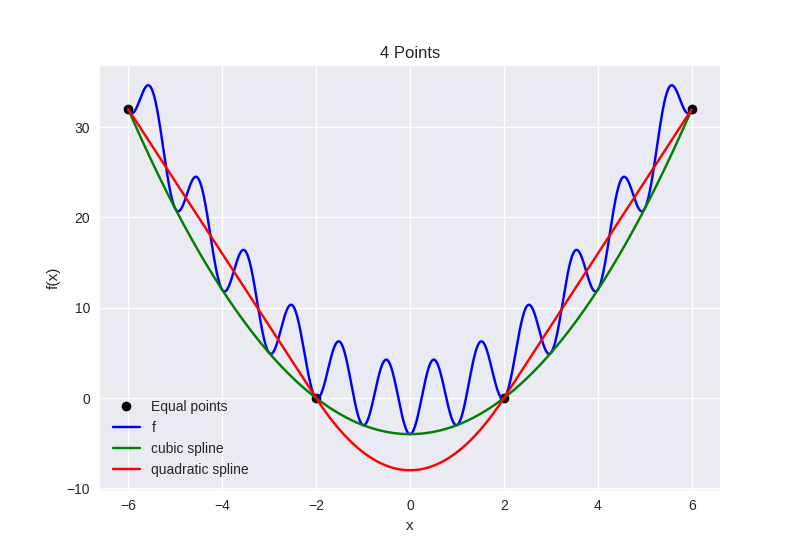
\includegraphics[width=\textwidth]{img/spline_4.png}
    \caption{Interpolacja splajnami dla 4 punktów}
\end{figure}

\begin{figure}[H]
    \centering
    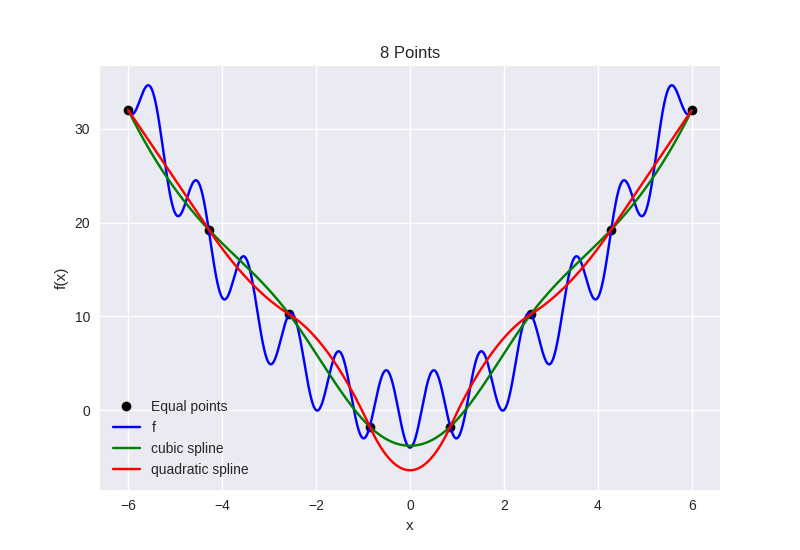
\includegraphics[width=\textwidth]{img/spline_8.png}
    \caption{Interpolacja splajnami dla 8 punktów}
\end{figure}

Dla 9 węzłów w przypadku wielomianów drugiego stopnia pojawiają się oscylacje, może być to spowodowane
wachającymi się wartościami funkcji w węzłach. Warto również zauważyć, że oscylacja występuje po prawej stronie wykresu, 
ponieważ dla lewego krańca określony jest warunek brzegowy. W przypadku wielomianów 3 stopnia podobny problem nie występuje.

\begin{figure}[H]
    \centering
    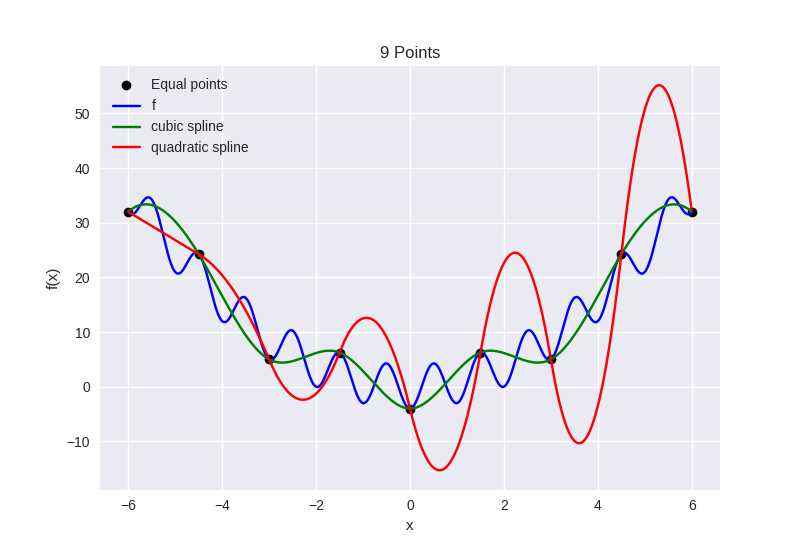
\includegraphics[width=0.8\textwidth]{img/spline_9.png}
    \caption{Interpolacja splajnami dla 9 punktów}
\end{figure}

\begin{figure}[H]
    \centering
    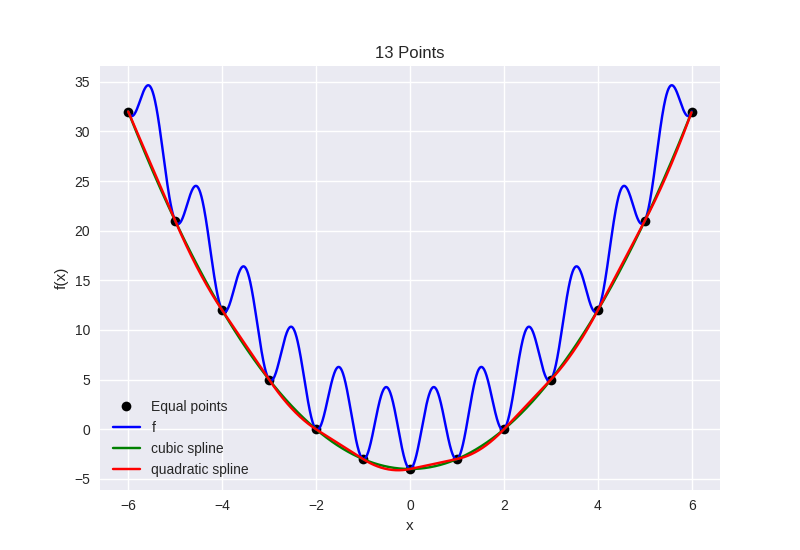
\includegraphics[width=0.8\textwidth]{img/spline_13.png}
    \caption{Interpolacja splajnami dla 13 punktów}
\end{figure}

Dla kolejnych liczb węzłów (większych niż 9) efekt oscylacji nie pojawia się, wielomiany zachowują się przewidywalnie.
Podobny problem pojawia się w okolicy liczby 22 węzłów. Tutaj, z racji dużej liczby węzłów, warunek brzegowy nieznacznie wpływa na obszar oscylacji.
Dla wielomianów 3 stopnia, podobnie jak w poprzednim przypadku, efekt nie występuje, poprawnie przybliżają badaną funkcję.

\begin{figure}[H]
    \centering
    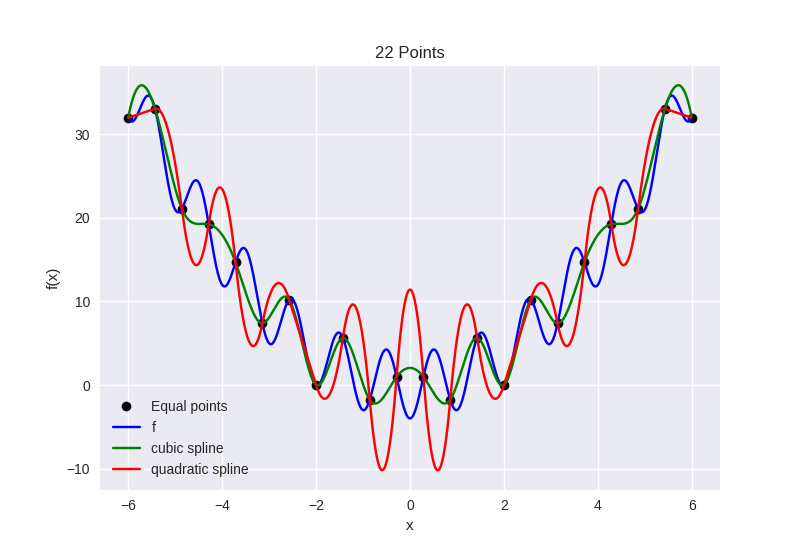
\includegraphics[width=0.8\textwidth]{img/spline_22.png}
    \caption{Interpolacja splajnami dla 22 punktów}
\end{figure}

\begin{figure}[H]
    \centering
    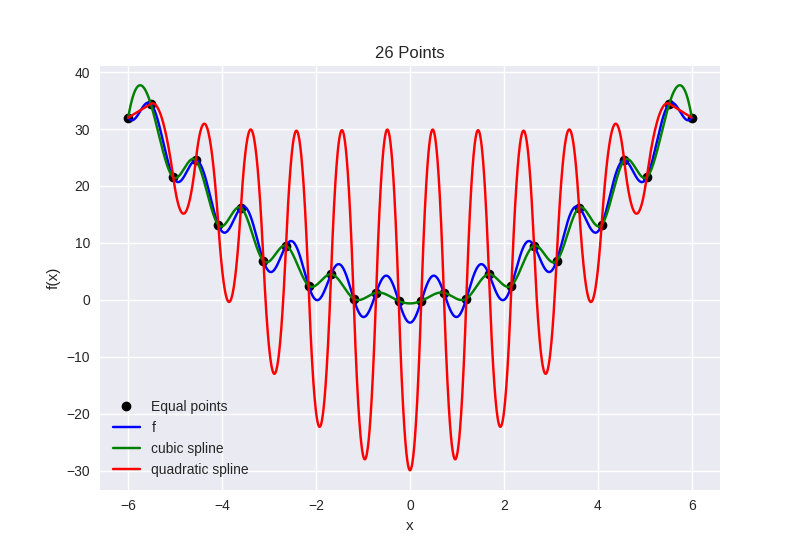
\includegraphics[width=0.8\textwidth]{img/spline_26.png}
    \caption{Interpolacja splajnami dla 26 punktów}
\end{figure}

Oscylacja nasila się do liczby 26 węzłów, następnie efekt maleje, a wielomniany drugiego stopnia coraz lepiej przybliżają badaną funkcję.

\begin{figure}[H]
    \centering
    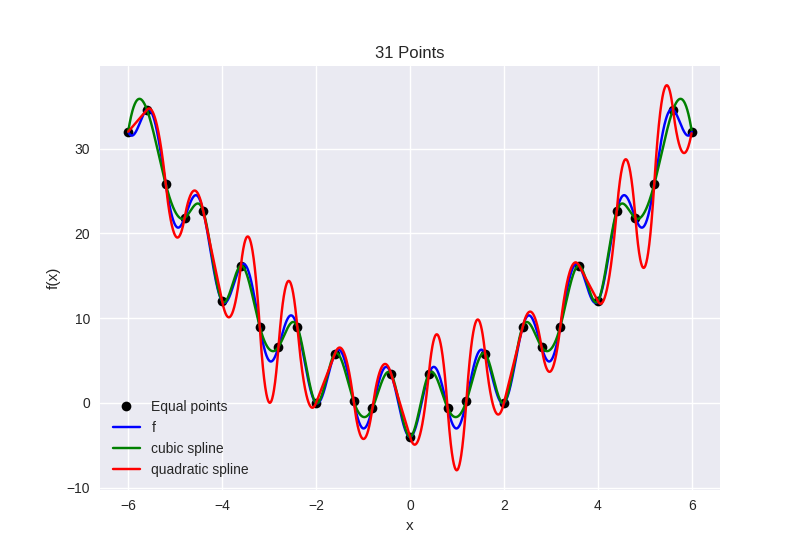
\includegraphics[width=\textwidth]{img/spline_31.png}
    \caption{Interpolacja splajnami dla 31 punktów}
\end{figure}

\begin{figure}[H]
    \centering
    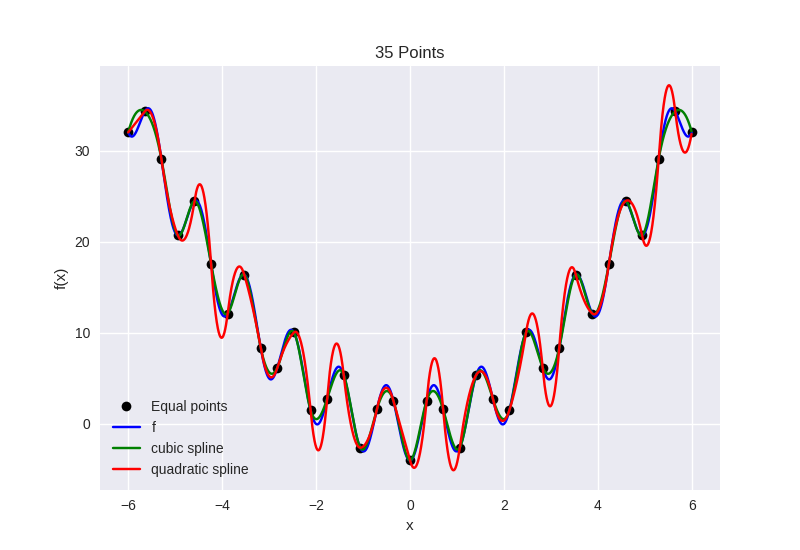
\includegraphics[width=\textwidth]{img/spline_35.png}
    \caption{Interpolacja splajnami dla 35 punktów}
\end{figure}

Na wykresie dla 35 punktów można zauważyć, że przybliżenie jest relatywnie dokładne dla wielomianów trzeciego stopnia oraz niewiele mniej dokładne
dla wielomianów drugiego stopnia.

\begin{figure}[H]
    \centering
    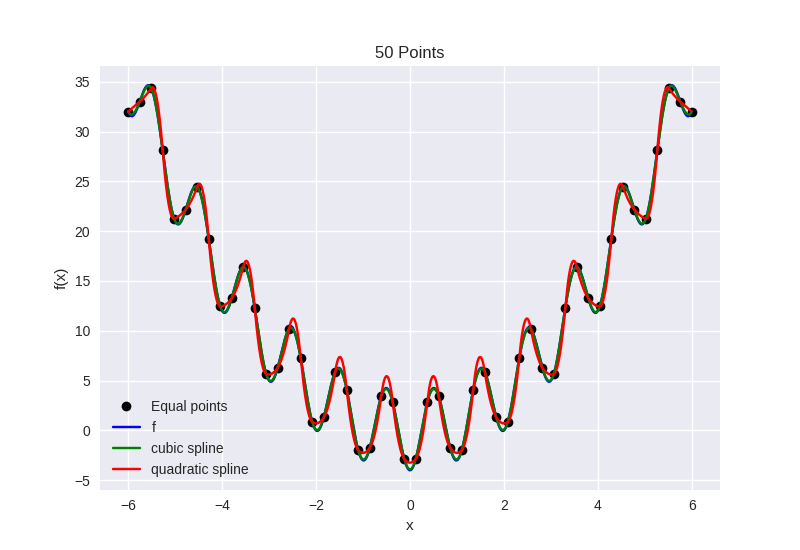
\includegraphics[width=\textwidth]{img/spline_50.png}
    \caption{Interpolacja splajnami dla 50 punktów}
\end{figure}

\subsection{Warunki brzegowe}
Zarówno dla wielomianów interpolowanych sklejanymi funkcjami trzeciego jak i drugiego stopnia zbadano dwa rodzaje warunków brzegowych:
\begin{itemize}
    \item
    dla wielomianów trzeciego stopnia:
    \begin{itemize}
        \item
        warunek 1 - przybliżanie trzecich pochodnych w pierwszym i ostatnim węźle ilorazami różnicowymi,
        wyprowadzony na wykładzie,
        \item
        warunek 2, free boundary - drugie pochodne w pierwszym i ostatnim węźle zastąpione zerami,
        $\sigma_0 = 0$ oraz $\sigma_{n} = 0$, ponieważ (z wykładu) $\sigma_i = \frac{1}{6}s''(x_i)$,
        gdzie $\sigma_i$ dla $i\in\{1..n\}$ są szukanymi.
    \end{itemize}
    \item
    dla wielomianów drugiego stopnia:
    \begin{itemize}
        \item
        warunek 1 - zastąpienie drugiej pochodnej w pierwszym węźle zerem.
        Bazując na wzorach z sekcji 1.1:
        \[s''_i=2c_i \land s''_0 = 0 \implies c_0 = 0\]
        wówczas wiersz macieży oznaczony pytajnikami będzie wyglądał następująco
        \[
        \begin{bmatrix}
        0 & 0 & 1 & 0 & \hdots & 0 \\
        \end{bmatrix}
        \times
        \hdots
        =
        \begin{bmatrix}
        0
        \end{bmatrix}
        \]
        \item
        warunek 2 - przybliżanie drugiej pochodnej w pierwszym węźle ilorazem różnicowymi:
        \[\Delta_i^{(1)} = \frac{y_{i+1} - y_i}{x_{i+1} - x_i}\]
        \[\Delta_i^{(2)} = \frac{\Delta_{i+1}^{(1)} - \Delta_{i}^{(1)}}{x_{i+2}-x_i}\]
        \[2s''_i(x) \approx 2\Delta_i^{(2)} \implies c_0 \approx \Delta_0^{(2)} = \frac{\frac{y_2-y_1}{x_2-x_1}-\frac{y_1-y_0}{x_1-x_0}}{x_2-x_0}\]
        wówczas wiersz macieży oznaczony pytajnikami będzie wyglądał następująco
        \[
        \begin{bmatrix}
        0 & 0 & 1 & 0 & \hdots & 0 \\
        \end{bmatrix}
        \times
        \hdots
        =
        \begin{bmatrix}
        \frac{\frac{y_2-y_1}{x_2-x_1}-\frac{y_1-y_0}{x_1-x_0}}{x_2-x_0}
        \end{bmatrix}
        \]
    \end{itemize}
\end{itemize}

Rozpocznijmy od zbadania zachowania wielomianów interpolowanych funkcjami sklejanymi trzeciego stopnia.

\begin{figure}[H]
    \centering
    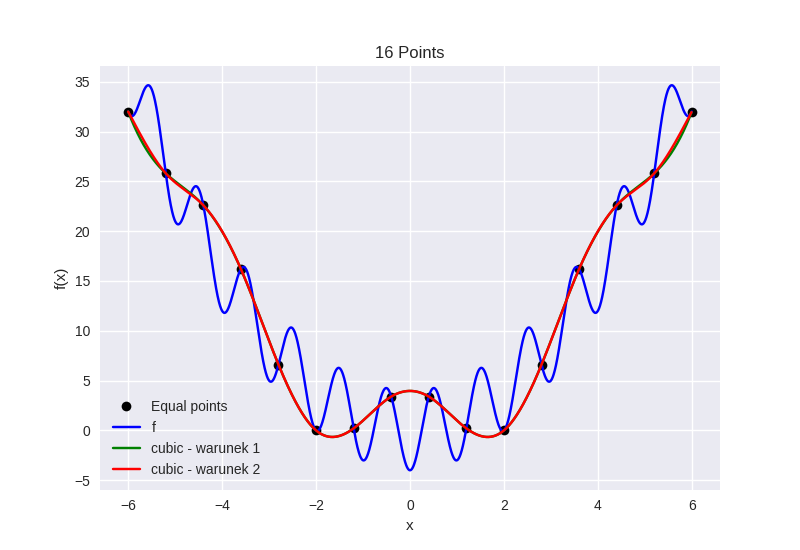
\includegraphics[width=0.9\textwidth]{img/cubic_16.png}
    \caption{Interpolacja funkcjami trzeciego stopnia dla 16 punktów}
\end{figure}

\begin{figure}[H]
    \centering
    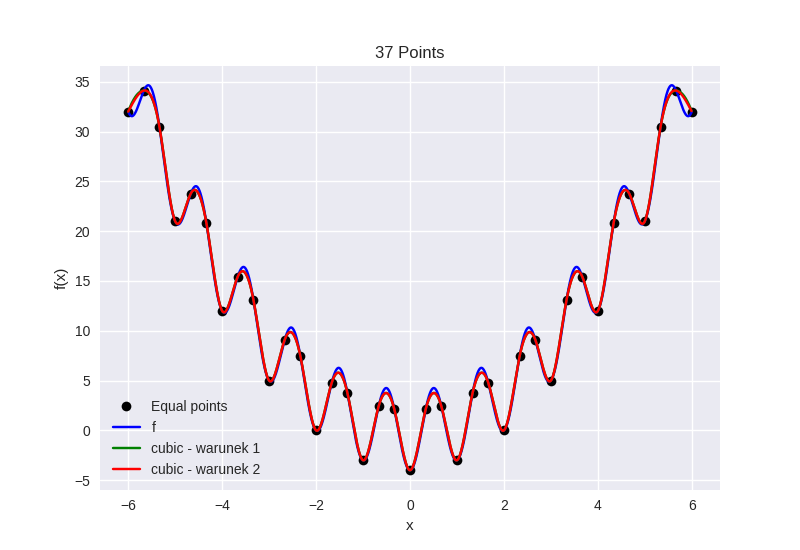
\includegraphics[width=0.9\textwidth]{img/cubic_37.png}
    \caption{Interpolacja funkcjami trzeciego stopnia dla 37 punktów}
\end{figure}

\newpage
Dla powyższych przypadków różnice są marginalne, jednak pojawiają się również takie, gdzie, w zależności od warunku, 
funkcja zachowuje się inaczej.

\begin{figure}[H]
    \centering
    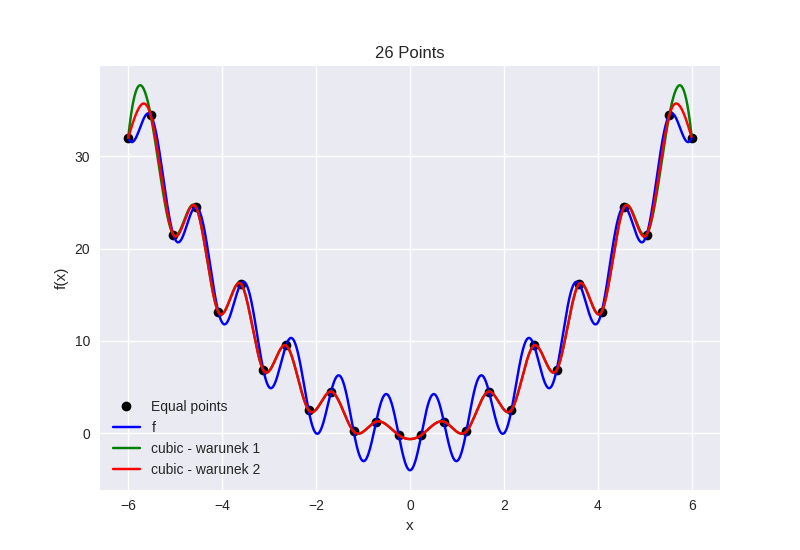
\includegraphics[width=\textwidth]{img/cubic_26.png}
    \caption{Interpolacja funkcjami trzeciego stopnia dla 26 punktów}
\end{figure}

W zakresie ok. 21-30 węzłów funkcja wygenerowana z wykorzystaniem warunku 1 osiąga większą wartość w maksimach lokalnych przy krańcach przedziału
niż dla warunku 2, jest mniej gładka. Podobny efekt, jednak z mniejszym natężeniem, można zaobserwować dla dużych liczb węzłów, np. 48-50. gdzie
z kolei funkcja dla warunku 1 osiąga mniejsze wartości w minimach przy krańcach przedziału, niż dla warunku 2. Generalnie, funkcje dla warunku 2
są bardziej gładkie przy krańcach przedziału.

\begin{figure}[H]
    \centering
    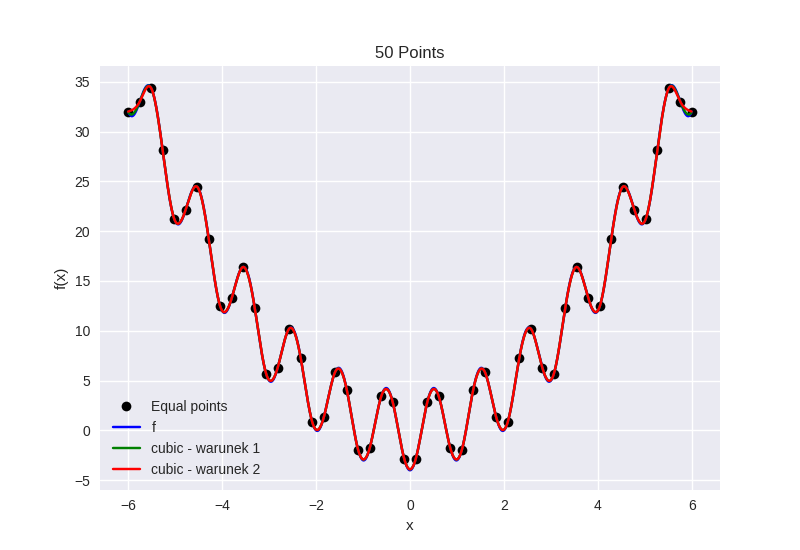
\includegraphics[width=\textwidth]{img/cubic_50.png}
    \caption{Interpolacja funkcjami 3 stopnia dla 50 punktów}
\end{figure}

Natomiast w przypadku wielomianów interpolowanych funkcjami sklejanymi drugiego stopnia dla niewielkich liczb węzłów 
można zauważyć istotne różnice w wykresach funkcji dla różnych warunków:

\begin{figure}[H]
    \centering
    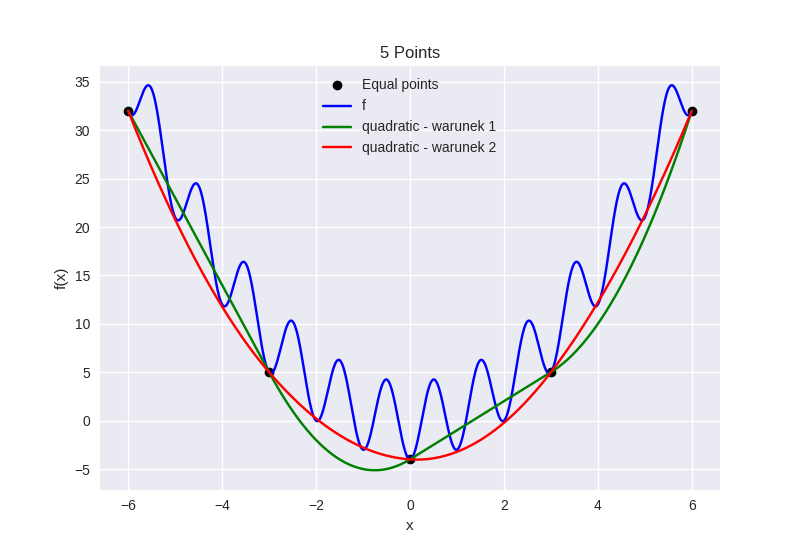
\includegraphics[width=\textwidth]{img/quadratic_5.png}
    \caption{Interpolacja funkcjami 2 stopnia dla 5 punktów}
\end{figure}

\begin{figure}[H]
    \centering
    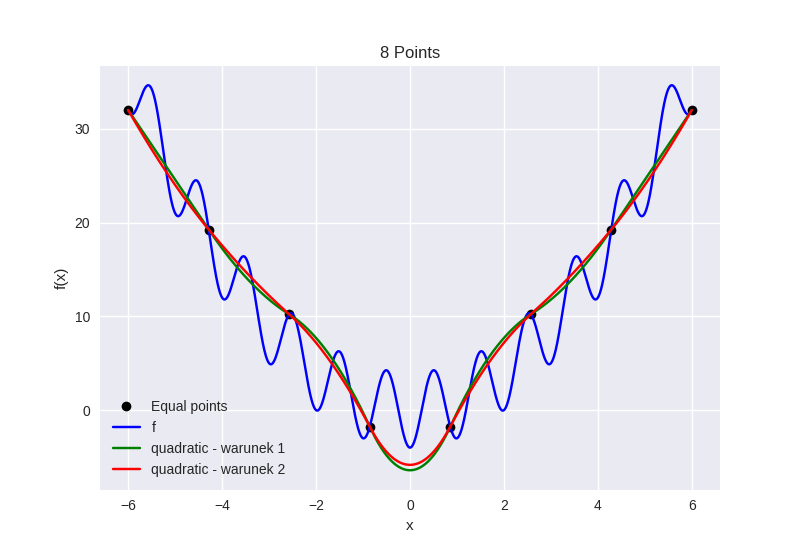
\includegraphics[width=\textwidth]{img/quadratic_8.png}
    \caption{Interpolacja funkcjami 2 stopnia dla 8 punktów}
\end{figure}

Jednak dla od pewnej liczby węzłów (ok. 8) wykresy funckcji interpolowanych wielomianami drugiego stopnia stają się bardzo podobne niezależnie od warunku.
Poniżej wykresy praktycznie całkowicie się pokrywają.

\begin{figure}[H]
    \centering
    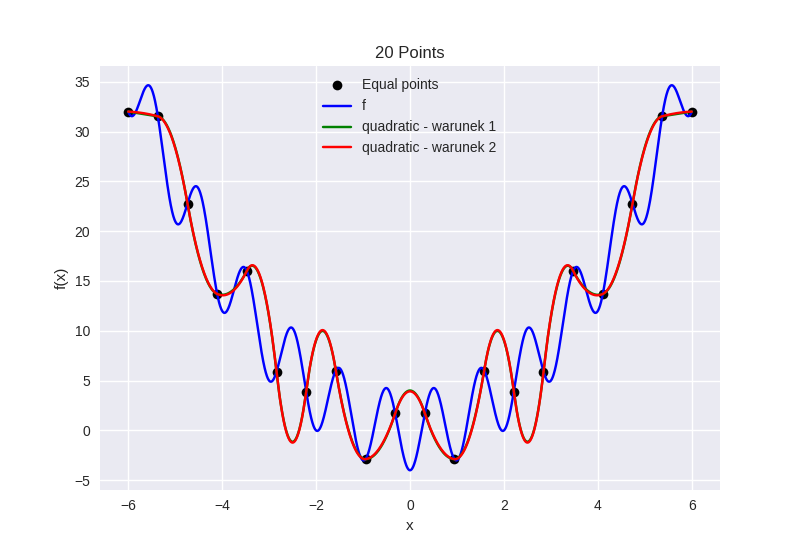
\includegraphics[width=\textwidth]{img/quadratic_20.png}
    \caption{Interpolacja funkcjami 2 stopnia dla 20 punktów}
\end{figure}

Jak można zaobserwować, w przypadku wielomianów 2 stopnia warunek brzegowy ma niewielki wpływ na funkcje sklejane dla większych liczb węzłów.

\subsection{Dokładność}
Pozostaje obliczenie dokładności oraz skonfrontowanie wyników z wnioskami uzyskanymi na podstawie analizy wykresów. Miarami dokładności będą:
\begin{itemize}
    \item
    średnia kwadratów odległości wartości wielomianu oraz funkcji $f$ dla 1000 równo oddalonych punktów,
    \item
    maksymalna odległość wartości wielomianu oraz funkcji $f$ dla 1000 równo oddalonych punktów.
\end{itemize}

Dla funkcji sklejanych interpolowanych wielomianami trzeciego stopnia:

\begin{table}[H]
\centering
\begin{tabular}{|l|ll|ll|}
\hline
\multirow{2}{*}{\begin{tabular}[c]{@{}l@{}}Liczba\\ węzłów\end{tabular}} & \multicolumn{2}{l|}{Śred. kwadratów} & \multicolumn{2}{l|}{Maks. odległości} \\ \cline{2-5} 
  & \multicolumn{1}{l|}{war. 1} & war. 2 & \multicolumn{1}{l|}{war. 1} & war. 2 \\ \hline
4 & \multicolumn{1}{l|}{23.976}    & 20.688   & \multicolumn{1}{l|}{8.000}   & 8.750    \\ \hline
5 & \multicolumn{1}{l|}{23.976}   & 22.394    & \multicolumn{1}{l|}{8.000}    & 8.159    \\ \hline
6 & \multicolumn{1}{l|}{12.348}   & 12.269    & \multicolumn{1}{l|}{7.326}    & 7.060    \\ \hline
7 & \multicolumn{1}{l|}{23.976}   & 23.451    & \multicolumn{1}{l|}{8.000}    & 8.093    \\ \hline
8 & \multicolumn{1}{l|}{14.922}   & 14.353    & \multicolumn{1}{l|}{7.812}    & 7.736    \\ \hline
9 & \multicolumn{1}{l|}{16.951}   & 15.484    & \multicolumn{1}{l|}{9.239}    & 7.691    \\ \hline
10 & \multicolumn{1}{l|}{13.882}   & 13.907    & \multicolumn{1}{l|}{7.510}    & 7.510    \\ \hline
11 & \multicolumn{1}{l|}{15.939}   & 15.439    & \multicolumn{1}{l|}{7.959}    & 7.995    \\ \hline
12 & \multicolumn{1}{l|}{15.992}   & 15.819    & \multicolumn{1}{l|}{7.996}    & 7.995    \\ \hline
13 & \multicolumn{1}{l|}{23.976}   & 23.893    & \multicolumn{1}{l|}{8.000}    & 8.024    \\ \hline
14 & \multicolumn{1}{l|}{15.988}   & 15.876    & \multicolumn{1}{l|}{7.997}    & 7.997    \\ \hline
15 & \multicolumn{1}{l|}{15.993}   & 15.766    & \multicolumn{1}{l|}{7.992}    & 7.987    \\ \hline
16 & \multicolumn{1}{l|}{15.880}   & 15.535    & \multicolumn{1}{l|}{7.959}    & 7.987    \\ \hline
17 & \multicolumn{1}{l|}{15.449}   & 15.116    & \multicolumn{1}{l|}{6.088}    & 6.115    \\ \hline
18 & \multicolumn{1}{l|}{14.594}   & 14.436    & \multicolumn{1}{l|}{7.741}    & 7.741    \\ \hline
19 & \multicolumn{1}{l|}{13.364}   & 13.440    & \multicolumn{1}{l|}{7.506}    & 7.505    \\ \hline
20 & \multicolumn{1}{l|}{11.914}   & 12.124    & \multicolumn{1}{l|}{7.131}    & 7.131    \\ \hline
21 & \multicolumn{1}{l|}{10.403}   & 10.551    & \multicolumn{1}{l|}{6.643}    & 6.642    \\ \hline
22 & \multicolumn{1}{l|}{8.934}   & 8.842    & \multicolumn{1}{l|}{6.041}    & 6.041    \\ \hline
23 & \multicolumn{1}{l|}{7.549}   & 7.144    & \multicolumn{1}{l|}{5.367}    & 5.370    \\ \hline
24 & \multicolumn{1}{l|}{6.259}   & 5.585    & \multicolumn{1}{l|}{4.697}    & 4.674    \\ \hline
25 & \multicolumn{1}{l|}{1.081}   & 0.254    & \multicolumn{1}{l|}{5.014}    & 2.443    \\ \hline
26 & \multicolumn{1}{l|}{4.021}   & 3.165    & \multicolumn{1}{l|}{5.076}    & 3.374    \\ \hline
27 & \multicolumn{1}{l|}{3.117}   & 2.326    & \multicolumn{1}{l|}{4.942}    & 2.825    \\ \hline
28 & \multicolumn{1}{l|}{2.372}   & 1.696    & \multicolumn{1}{l|}{4.669}    & 2.529    \\ \hline
29 & \multicolumn{1}{l|}{1.778}   & 1.234    & \multicolumn{1}{l|}{4.319}    & 2.430    \\ \hline
30 & \multicolumn{1}{l|}{1.318}   & 0.900    & \multicolumn{1}{l|}{3.929}    & 2.301    \\ \hline
31 & \multicolumn{1}{l|}{0.969}   & 0.660    & \multicolumn{1}{l|}{3.526}    & 2.163    \\ \hline
32 & \multicolumn{1}{l|}{0.709}   & 0.488    & \multicolumn{1}{l|}{3.141}    & 2.018    \\ \hline
33 & \multicolumn{1}{l|}{0.517}   & 0.364    & \multicolumn{1}{l|}{2.773}    & 1.880    \\ \hline
34 & \multicolumn{1}{l|}{0.376}   & 0.274    & \multicolumn{1}{l|}{2.433}    & 1.747    \\ \hline
\end{tabular}
\caption{Dokładności dla wielomianów trzeciego stopnia}
\end{table}

Dla wielomianów trzeciego stopnia dokładności są bardzo podobne z niewielkimi wyjątkami np. w okolicach liczby 26 węzłów, gdzie
miara maksymalnej odległości pomiędzy punktami rzeczywistej funkcji a funkcji sklejanej odzwierciedla zjawisko opisane na 
stronie 8.

\begin{table}[H]
\centering
\begin{tabular}{|l|ll|ll|}
\hline
\multirow{2}{*}{\begin{tabular}[c]{@{}l@{}}Liczba\\ węzłów\end{tabular}} & \multicolumn{2}{l|}{Śred. kwadratów} & \multicolumn{2}{l|}{Maks. odległości} \\ \cline{2-5} 
    & \multicolumn{1}{l|}{war. 1} & war. 2 & \multicolumn{1}{l|}{war. 1} & war. 2 \\ \hline
4 & \multicolumn{1}{l|}{25.262}    & 25.014   & \multicolumn{1}{l|}{11.751}   & 8.469    \\ \hline
5 & \multicolumn{1}{l|}{26.673}   & 24.009    & \multicolumn{1}{l|}{10.250}    & 8.250    \\ \hline
6 & \multicolumn{1}{l|}{13.946}   & 16.113    & \multicolumn{1}{l|}{7.399}    & 8.222    \\ \hline
7 & \multicolumn{1}{l|}{24.509}   & 23.981    & \multicolumn{1}{l|}{8.753}    & 8.075    \\ \hline
8 & \multicolumn{1}{l|}{16.511}   & 16.257    & \multicolumn{1}{l|}{9.161}    & 8.761    \\ \hline
9 & \multicolumn{1}{l|}{152.841}   & 154.855    & \multicolumn{1}{l|}{30.441}    & 30.573    \\ \hline
10 & \multicolumn{1}{l|}{17.466}   & 17.331    & \multicolumn{1}{l|}{10.941}    & 10.713    \\ \hline
11 & \multicolumn{1}{l|}{16.692}   & 16.376    & \multicolumn{1}{l|}{9.140}    & 8.804    \\ \hline
12 & \multicolumn{1}{l|}{15.813}   & 15.909    & \multicolumn{1}{l|}{7.909}    & 7.865    \\ \hline
13 & \multicolumn{1}{l|}{24.009}   & 23.976    & \multicolumn{1}{l|}{8.250}    & 8.023    \\ \hline
14 & \multicolumn{1}{l|}{15.865}   & 15.946    & \multicolumn{1}{l|}{8.326}    & 8.095    \\ \hline
15 & \multicolumn{1}{l|}{16.272}   & 16.177    & \multicolumn{1}{l|}{8.581}    & 8.389    \\ \hline
16 & \multicolumn{1}{l|}{16.266}   & 16.239    & \multicolumn{1}{l|}{8.938}    & 8.794    \\ \hline
17 & \multicolumn{1}{l|}{17.821}   & 17.720    & \multicolumn{1}{l|}{7.459}    & 7.376    \\ \hline
18 & \multicolumn{1}{l|}{18.279}   & 18.263    & \multicolumn{1}{l|}{9.918}    & 9.893    \\ \hline
19 & \multicolumn{1}{l|}{22.025}   & 22.083    & \multicolumn{1}{l|}{10.610}    & 10.644    \\ \hline
20 & \multicolumn{1}{l|}{23.873}   & 23.925    & \multicolumn{1}{l|}{11.435}    & 11.519    \\ \hline
21 & \multicolumn{1}{l|}{33.679}   & 33.942    & \multicolumn{1}{l|}{12.989}    & 13.115    \\ \hline
22 & \multicolumn{1}{l|}{43.049}   & 42.921    & \multicolumn{1}{l|}{15.408}    & 15.564    \\ \hline
23 & \multicolumn{1}{l|}{90.338}   & 90.737    & \multicolumn{1}{l|}{20.369}    & 20.546    \\ \hline
24 & \multicolumn{1}{l|}{251.218}   & 247.394    & \multicolumn{1}{l|}{31.368}    & 31.180    \\ \hline
25 & \multicolumn{1}{l|}{1533.187}   & 1523.763    & \multicolumn{1}{l|}{91.909}    & 91.717    \\ \hline
26 & \multicolumn{1}{l|}{173.490}   & 170.268    & \multicolumn{1}{l|}{25.912}    & 25.720    \\ \hline
27 & \multicolumn{1}{l|}{46.838}   & 47.260    & \multicolumn{1}{l|}{14.855}    & 15.042    \\ \hline
28 & \multicolumn{1}{l|}{15.441}   & 15.514    & \multicolumn{1}{l|}{9.847}    & 10.026    \\ \hline
29 & \multicolumn{1}{l|}{10.174}   & 10.539    & \multicolumn{1}{l|}{7.380}    & 7.548    \\ \hline
30 & \multicolumn{1}{l|}{5.348}   & 5.591    & \multicolumn{1}{l|}{5.888}    & 6.045    \\ \hline
31 & \multicolumn{1}{l|}{4.512}   & 4.809    & \multicolumn{1}{l|}{4.938}    & 5.083    \\ \hline
32 & \multicolumn{1}{l|}{2.988}   & 3.218    & \multicolumn{1}{l|}{4.246}    & 4.378    \\ \hline
33 & \multicolumn{1}{l|}{2.758}   & 2.990    & \multicolumn{1}{l|}{3.594}    & 3.714    \\ \hline
34 & \multicolumn{1}{l|}{2.084}   & 2.272    & \multicolumn{1}{l|}{3.330}    & 3.439    \\ \hline
\end{tabular}
\caption{Dokładności dla wielomianów drugiego stopnia}
\end{table}

W przypadku wielomianów drugiego stopnia wyniki potwierdzają tezę, że wybór warunku (spośród dwóch
przedstawionych tutaj) nie ma dużego wpływu na dokładność. Widoczne są również spadki dokładności wynikające z oscylacji
opisanych na stronie 4.

\newpage
\begin{table}[H]
\centering
\begin{tabular}{|l|l|l|}
\hline
Liczba węzłów & wiel. 2 stopnia, war. 2 & wiel. 3 stopnia, war. 1\\ \hline
4 & 25.014    & 23.976     \\ \hline
5 & 24.009      & 23.976    \\ \hline
6 & 16.113    & 12.348    \\ \hline
7 & 23.981    & 23.976    \\ \hline
8 & 16.257    & 14.922    \\ \hline
9  & 154.855      & 16.951    \\ \hline
10 & 17.331      & 13.882    \\ \hline
11 & 16.376     & 15.939     \\ \hline
12 & 15.909     & 15.992     \\ \hline
13 & 23.976     & 23.976    \\ \hline
14 & 15.946     & 15.988    \\ \hline
15 & 16.177     & 15.993    \\ \hline
16 & 16.239     & 15.880    \\ \hline
17 & 17.720     & 15.449     \\ \hline
18 & 18.263     & 14.594    \\ \hline
19 & 22.083      & 13.364   \\ \hline
20 & 23.925      & 11.914    \\ \hline
21 & 33.942      & 10.403    \\ \hline
22 & 42.921      & 8.934     \\ \hline
23 & 90.737      & 7.549    \\ \hline
24  & 247.394      & 6.259    \\ \hline
25   & 1523.763    & 1.081    \\ \hline
26  & 170.268      & 4.021    \\ \hline
27 & 47.260      & 3.117    \\ \hline
28 & 15.514     & 2.372    \\ \hline
29 & 10.539     & 1.778     \\ \hline
30& 5.591     & 1.318    \\ \hline
31& 4.809     &   0.969   \\ \hline
32& 3.218     &  0.709   \\ \hline
33& 2.990     & 0.517   \\ \hline
34& 2.272     &  0.376   \\ \hline
\end{tabular}
\caption{Średnie kwadratów odległości dla wielomianów}
\end{table}

Dla obu metod wybrane zostały warunki brzegowe w jakiś sposób przybliżające wartość pochodnych wielomianu.
W ogólności interpolowanie funkcjami sklejanymi trzeciego stopnia konsekwentnie wykazuje lepszą dokładność oraz 
nie cierpi z powodu oscylacji. 

\newpage
\section{Wnioski}
Interpolacje funkcjami sklejanymi drugiego i trzeciego stopnia to skuteczne sposoby na przybliżanie funkcji, które pozwalają
na uniknięcie skutków używania wielomianów wysokich stopni (efekt Rungego), jak w metodach Lagrange'a czy Newtona. Ażeby skutecznie przybliżyć
funkcję splajnami przy większej liczbie węzłów, lepiej skorzystać z wielomianów trzeciego stopnia, które produkują gładszą funkcję
wynikową i nie cierpią z powodu oscylacji. Metody te wymagają również skrzystania z warunku brzegowego, np. "free boundary", które
są koniecznie do rozwiązania układu równań dostarczającego funkcję wynikową i mogą wpływać na dokładność przybliżenia w zależności
od liczby węzłów i wykorzystania.

\end{document}